% LaTeX file for CJFAS short communication paper (Hutchings, Minto, Ricard and Baum)
% DR CM Started 2010-01-12 from Jeff's RTF file
% Last modified Time-stamp: <Last modified: 19 JANUARY   (srdbadmin)>
%
\documentclass[letterpaper,12pt]{article}

\usepackage[authoryear]{natbib} 
\usepackage{url} 
\usepackage{graphicx}
\usepackage{lineno} 
\usepackage{paralist} 
\usepackage{comment}
\usepackage{url}
\usepackage{color}

%\linenumbers

\title{Convention on Biological Diversity 2010 Target and the
Biodiversity of Marine Fishes} 

\author{Jeffrey Hutchings
\thanks{Department of Biology, Dalhousie University, 1355 Oxford
Street, Halifax, NS B3H 4J1, Canada} \and C{\'o}il{\'i}n Minto$^{*}$
\and Daniel Ricard$^{*}$ \and Julia Baum\thanks{National Center for
Ecological Analysis and Synthesis (NCEAS), 735 State Street, Suite
300, Santa Barbara, CA 93101, USA} }



\begin{document}

\maketitle{}

\section*{Abstract} 
The Convention on Biological Diversity (CBD) ...

\section{Introduction} 
The United Nations has declared 2010 to be the
International Year of Biodiversity. This is a direct response to
initiatives by the Convention on Biological Diversity (CBD;
established 1993) to: (i) conserve biological diversity; (ii) use
biological diversity in a sustainable fashion; and (iii) share the
benefits of biological diversity fairly and equitably. In April 2002,
the Conference of the Parties adopted a strategic plan for the CBD,
the mission statement of which articulated what has become known as
the ``2010 Biodiversity Target'': to achieve by 2010 a significant
reduction of the current rate of biodiversity loss at the global,
regional and national level as a contribution to poverty alleviation
and to the benefit of all life on Earth
(\url{http://cbd.int/2010-target/about.shtml}).  

Among the indicators formally identified by the CBD to evaluate the
progress achieved in meeting the 2010 Biodiversity Target is one that examines
``trends in the abundance and distribution of selected species''. The
only index formally under consideration by the CBD that pertains to
marine fishes is the Marine Living Planet Index \citep{WWF:2008}.
Although it utilizes information on 162 fish species, these trend data have
not been segregated from those available on the other 179 species used
in the index.  Our objective here is to quantify trends in population
abundance and biomass to assess the degree to which the CBD's 2010 Biodiversity
Target is likely to be met for marine fishes on global and regional
scales. Our analysis extends the temporal, spatial, taxonomic, and
analytical breadth of the only previous global and regional
examination of populations trends in marine fishes
(\cite{Hutchings:Baum:2005:philtransB}; hereafter, HB2005).

\section{Materials and Methods} 
Data on spawning stock biomass (SSB) were compiled from stock
assessments undertaken by scientists associated with national and
international fisheries management agencies.  This database will soon
be made available to interested researchers
(\url{http://www.marinebiodiversity.ca/RAMlegacy/srdb}). The
geographical breadth of these data included: Northeast Pacific
(Eastern Bering Sea, Gulf of Alaska, British Columbia, California
Current); Northwest Atlantic (Northeast Newfoundland Shelf, Gulf of
St. Lawrence, Scotian Shelf, Bay of Fundy, Gulf of Maine, Georges
Bank, Northeast and Southeast U.S. Shelves, Gulf of Mexico); Northeast
Atlantic (Barents Sea, North Sea, Iceland, Irish Sea, Baltic Sea,
Faroes); Australia/New Zealand; South America; and South Africa. To
reduce variability in data quality, we restricted our analysis to
spawner biomass data estimated from age-structured, sequential
population analyses reported in fisheries stock assessments.  

\textcolor{red}{Given that the 2010 Biodiversity Target is a target based on the rate
of change in abundance, we compared the slopes of linear regressions
of log-transformed SSB plotted against time for two different time
periods. For each population/stock, we compared regression slopes for
all available data up to 1991 (the year the CBD was initially
agreed upon) with those for all available data from 1992 onwards
(usually to 2007). Our analyses were restricted to those stocks with a
minimum of 25 years of data dating back to 1978 or earlier.}

\textcolor{red}{
We estimated the slopes up to 1991 and the change in slopes observed
after 1992:}
\begin{equation}
log(SSB)_{y+1} = \alpha_{pre1992} + (\eta * \delta_{intercept}) +(slope_{pre1992}+(\eta * \delta_{slope}))y 
\end{equation}
where,
\begin{description}
\item[$\alpha$]{is the intercept}
\item[$\eta$]{is a class variable determining whether year $y$ is before ($\eta=0$) or after and including ($\eta=1$) 1992}
\item[$\delta_{intercept}$]{}
\item[$slope_{pre1992}$]{is the temporal slope up to to 1991}
\item[$\delta_{slope}$]{is the change in slope observed after 1992}
\end{description}

\textcolor{red}{
Under this model, a reduction in the rate of decline after 1992, reflected by a positive
slope difference (i.e., $\delta_{slope} > 0$),
would be consistent with the 2010 Biodiversity Target.
}

Multi-species indices of abundance were also constructed for those
stocks for which data were available for the 30-year period extending
from 1978 to 2007 (adopting the same starting year as HB2005 but
extending the time series from 2001 to 2007). For each stock, we
standardized the spawning stock biomass data by dividing the annual
estimates by the maximum recorded for each stock (SSBmax) and then
log-transformed the data. For each year between 1978 and 2007, the
multi-species index was calculated from the geometric mean across all
stocks.  To assist us in interpreting the results, we felt it would be
informative to compare the current total biomass and fishing mortality
experienced by each stock relative to those associated with target
reference points appropriate for each stock. The fishing mortality
data will be made available when the database contents are published. The
target reference points are BMSY and FMSY, which represent the
estimated total biomass and fishing mortality, respectively, at which
the maximum sustainable yield (MSY) can be achieved. These reference
points are those reported by \citet{Worm:etal:2009:science}. To conform with the
terminology used in the only national jurisdiction (U.S.) for which
overfishing and its associated management responses have been
articulated by legislation, a stock is experiencing overfishing when
 $F_{current} > F_{MSY}$  and a stock is in an overfished state when  $B_{current} < 0.5B_{MSY}$.

\section{Results} 
\textcolor{red}{
Globally, among the 114 stocks (65.5\% of all stocks examined) in
decline prior to 1992 ($slope_{pre1992} < 0$), the slope difference
for 66.7\% of these was positive, indicative of an easing of their
rates of decline after 1992. Regionally, the slope difference was
positive for all stocks in the Middle North Atlantic (100\% of 9
stocks), more than half the stocks in the Northwest Atlantic (85\% of
13 stocks), Northeast Atlantic (72\% of 25 stocks), Northeast Pacific
(75\% of 32 stocks) and South Africa (75\% of 4 stocks) (Figure 1a,
1b, 1c, 1d and 1f). By comparison, the slope difference was positive for
slightly less than half of the stocks in decline prior to 1992 in
Australia/New Zealand (45\% of 20 stocks) (Figure 1e).
}

\textcolor{red}{
Some stocks for which the rate of decline had lessened were still in
decline after 1992: 6 of 18 in the Northeast Atlantic; 5 of 24 in the
Northeast Pacific; 9 of 9 in Australia/New Zealand; and 1 of 3 in
South Africa.  For a number of stocks, their rate of decline increased
after 1992, the slope difference being negative for: 2 stocks in the
Northwest Atlantic; 7 in the Northeast Atlantic; 8 in the Northeast
Pacific; 11 in Australia/New Zealand; and 1 in South Africa.
}

Species for which the rate of decline increase after 1992
were generally those feeding at high trophic levels (defined as those
whose maximum trophic level, given by www.fishbase.org, exceeds 4.2),
such as Atlantic cod (\emph{Gadus morhua}), Plaice (\emph{Pleuronectes
  platessa}), Blue Whiting (\emph{Micromesistius poutassou}),
sablefish (\emph{Anoplopoma fibria}), rockfishes (\emph{Sebastes}
spp.), and Hoki (\emph{Macruronus novaezelandiae}).  

The multi-species abundance indices were based on abundance data for
142 stocks.  Based on data for all species globally, the multi-species
index declined 26\% from an average of 0.54SSBmax to 0.40SSBmax
(Figure~\ref{fig2}).  Distinguishing species by their primary
habitat/life style, the pattern of temporal change in the index
differed between pelagic and demersal species. The index for pelagic
species increased from the late 1970s through the mid 1980s (Fig. 2b).
Since reaching a peak between 1986 and 1988, the index has declining
steadily through 2007.  By contrast, the demersal species index peaked
at 0.65SSBmax during the earliest part of the time series before
declining steadily through the mid 1990s to a level ranging between
0.40 and 0.44SSBmax where it has remained through 2007, possibly
exhibiting signs of an increase in later years (Fig. 2b).

Regionally, pelagic species have been
increasing since 1978 in the Northeast Atlantic (N = 12 stocks) and
possibly the Northeast U.S.  (based on 2 stocks); overall, pelagics
have shown declines in the Canadian Atlantic (N = 4) and Australia/New
Zealand (N = 40) (Figs.  2c-f). With the exception of stability in
Australia/New Zealand, demersal species have shown declines throughout
the time series, with evidence of increases in the past decade in the
Northeastern U.S (N = 5 stocks) and possibly the Canadian Atlantic (N
= 15 stocks).

\section{Discussion} The present work represents a significant spatial
and temporal expansion of data considered in the only previous
analysis of changes in the rate of decline of marine fishes. Whereas
HB2005's data were limited primarily to North Atlantic and Canada's
Pacific waters, our study also included North America's entire Pacific
coast, the Mediterranean Sea, and the waters surrounding Australia and
New Zealand. Although our sample size was slightly less than the 177
considered previously, the present analysis was restricted to 157
stocks for which assessment-based estimates of SSB were
available. HB2005, whose data set included 103 SSB abundance-based
stocks, also analyzed trends in stocks for which only alternative
abundance metrics were available, e.g., fisheries-independent survey
catch rates. The multi-species abundance indices constructed here
include data current to 2007, extending those considered by HB2005 by
six years.  Most of the world's fish stocks assessed by national and
international agencies (66\%) were declining prior to 1992, a result
consistent with previous studies of marine fish abundance
\citep{Hutchings:2000:nature, Myers:Worm:2005:philtransB}. Since 1992,
the rate of decline has been reduced in 67\% of these stocks (N = 70),
a pattern consistent with the 2010 CBD Biodiversity Target. However,
for the remaining 33\% of stocks (N = 34), which represent species
feeding at the highest trophic levels, the rate of decline has
increased. The percentage of stocks whose trends conform with the 2010
Target reported here (67\%) is less than the 81\% reported by HB2005,
meaning that declines in marine fish biodiversity have not been
arrested to as great an extent as previously thought. (If one
restricts HB2005's analysis to the 103 stocks for which abundance data
were based only on SSB, 65\% of stocks would have conformed with the
2010 Target.)

Questions:
\begin{enumerate}
\item{Of those stocks in decline before 1992, and increasing since
1992, what is the current B and F relative Bmsy and Fmsy?}
\item{Of those stocks in decline before 1992, and declining at faster
rate since 1992, what is the current B and F relative Bmsy and Fmsy?}
\end{enumerate}



\section*{Acknowledgements} 
We are happy to acknowledge all those who
have contributed to the establishment of the RAM Legacy
Stock-Recruitment Database, notably the financial support provided by
a Natural Sciences and Engineering Research Council (NSERC) Discovery
Grant to JAH and monies allocated to a National Center for Ecological
Analysis and Synthesis (NCEAS) Working Group Project organized by Ray
Hilborn and Boris Worm. XX and XX provided very helpful comments on an
earlier version of the manuscript. The research was support by a NSERC
Discovery Grant to JAH. JKB was supported by a David H. Smith
Conservation Research Fellowship.

%\bibliographystyle{authordate1} 
\bibliographystyle{cjfas} 
\bibliography{./CJFAS-shortcomm}


\section*{Figures}
\subsection*{Figure legends}
\textcolor{red}{
\noindent Figure 1. Slope of the temporal trends of $log(SSB)$ as obtained by a linear model with no continuity constraint for stocks located in a) the Northwest Atlantic (n=13), b) the Northeast Atlantic (n=25), c) the Middle North Atlantic (n=9), d) the Northeast Pacific (n=32), e) Australia and New Zealand (n=20) and f) South Africa (n=4). Open triangles represent the temporal slope prior to 1992, solid black triangles represent the temporal slope after 1992 and solid red triangles represent the difference in slope before- and after-1992. For each region, the stocks are ordered by the difference in slope before- and after-1992. The slope value represents the annual rate of change in population biomass.}\\

\noindent Figure 2. \\

\subsection*{Figures}

\begin{figure}\label{fig1}
\begin{center}
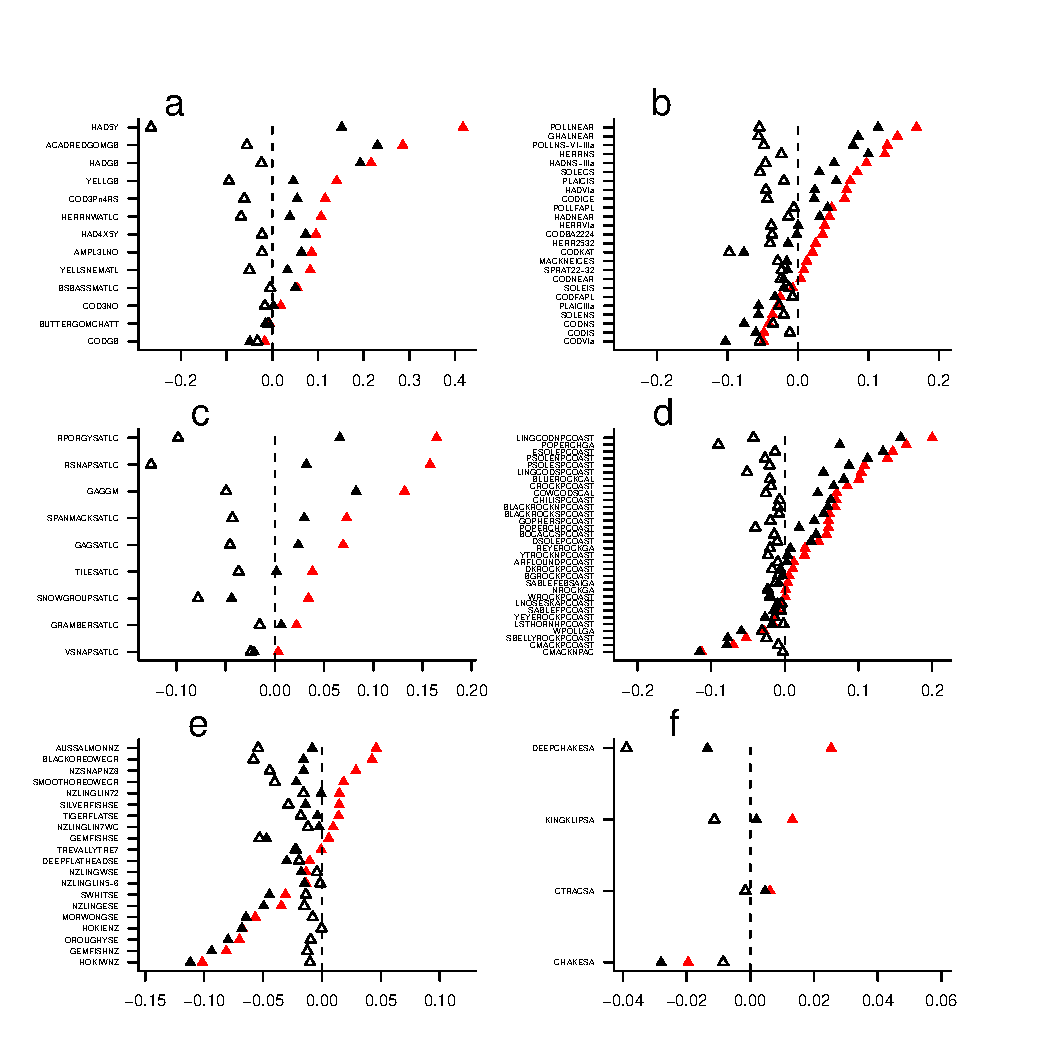
\includegraphics[width=17cm]{/home/srdbadmin/SQLpg/srdb/trunk/projects/baumhutchings/R/CJFAS-shortcomm-fig1.pdf}
\end{center}
\caption{}
\end{figure}

%\begin{figure}
%\begin{center}
%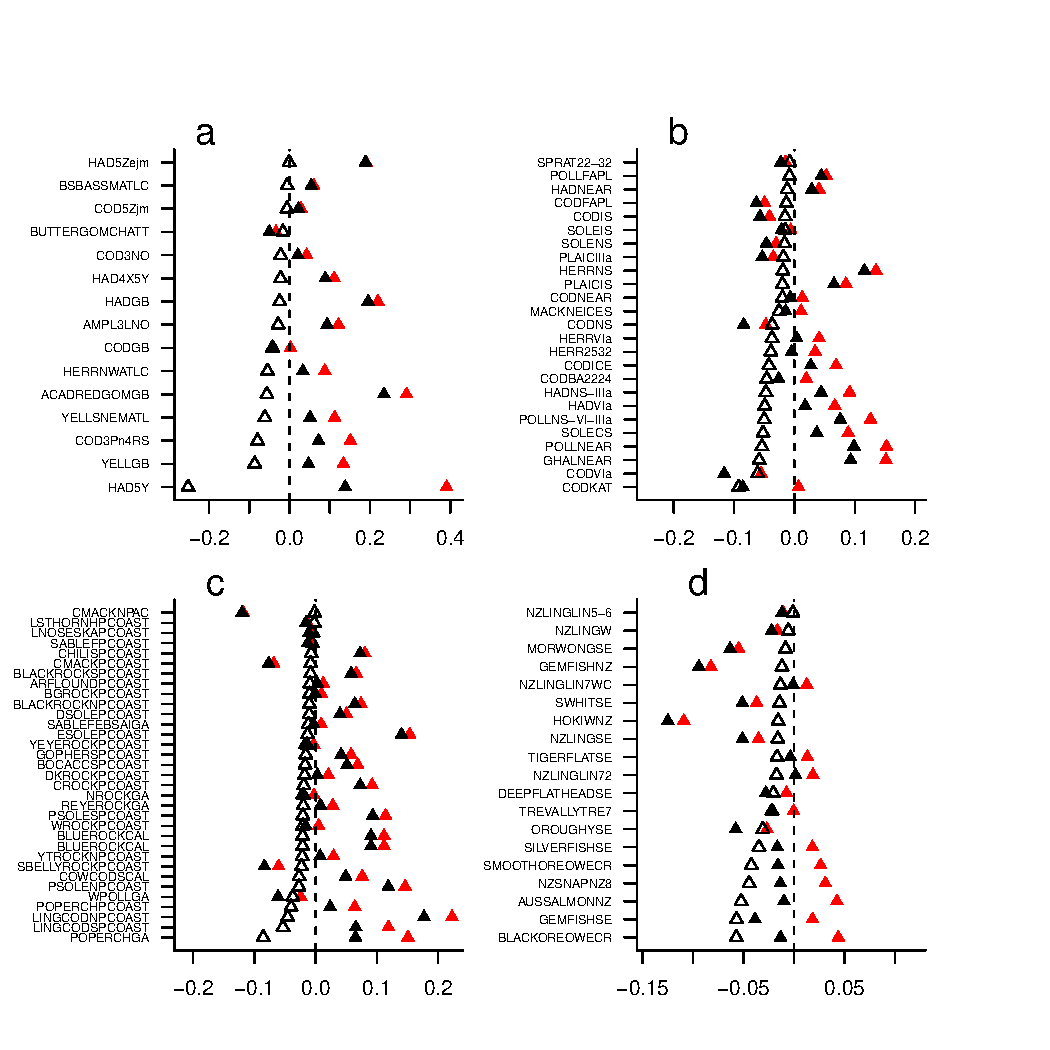
\includegraphics[height=17cm]{/home/srdbadmin/SQLpg/srdb/trunk/projects/baumhutchings/R/CJFAS-shortcomm-fig1-orderedbypreslope.pdf}
%\end{center}
%\caption{ordered by pre-1992 slope value}
%\end{figure}

%\begin{figure}
%\begin{center}
%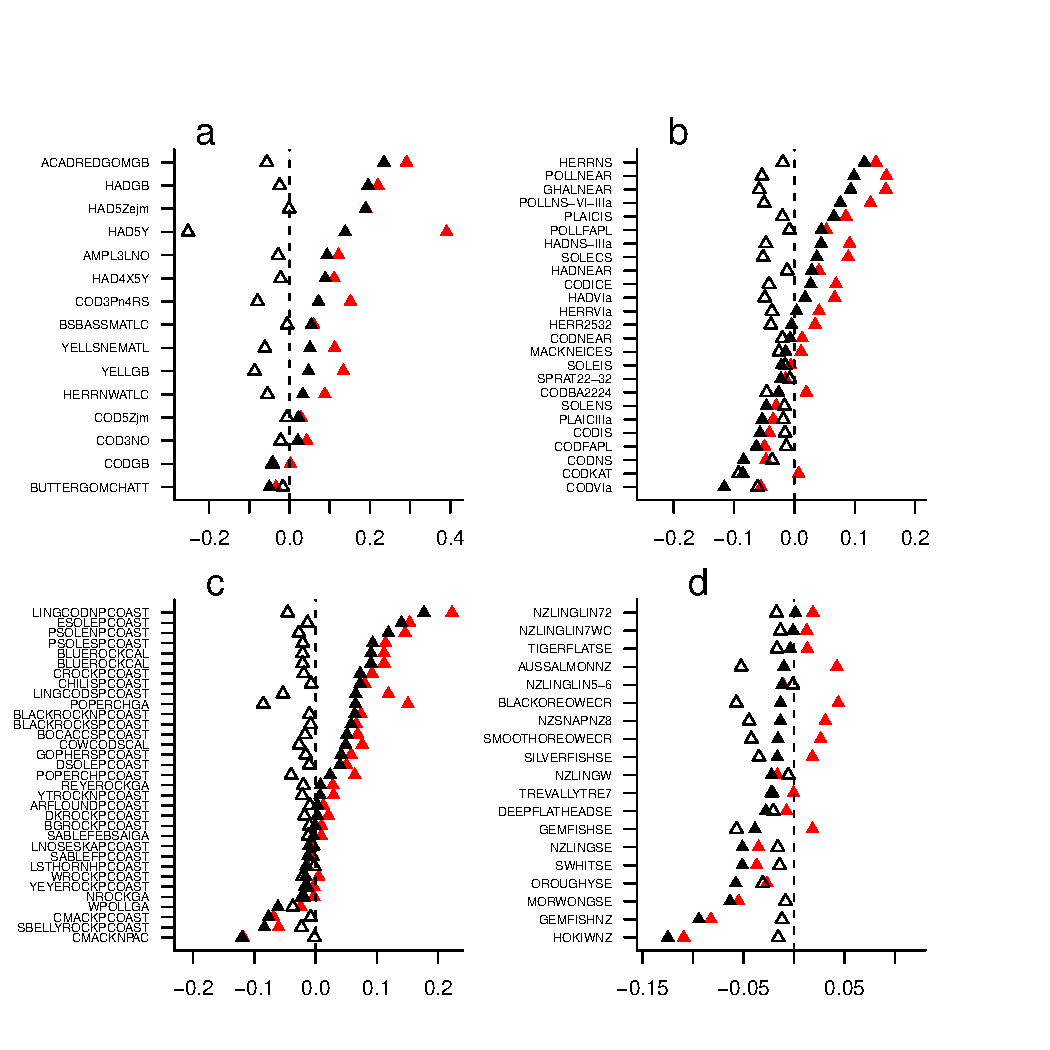
\includegraphics[height=17cm]{/home/srdbadmin/SQLpg/srdb/trunk/projects/baumhutchings/R/CJFAS-shortcomm-fig1-orderedbypostslope.pdf}
%\end{center}
%\caption{ordered by post-1992 slope value}
%\end{figure}

\begin{figure}
\begin{center}
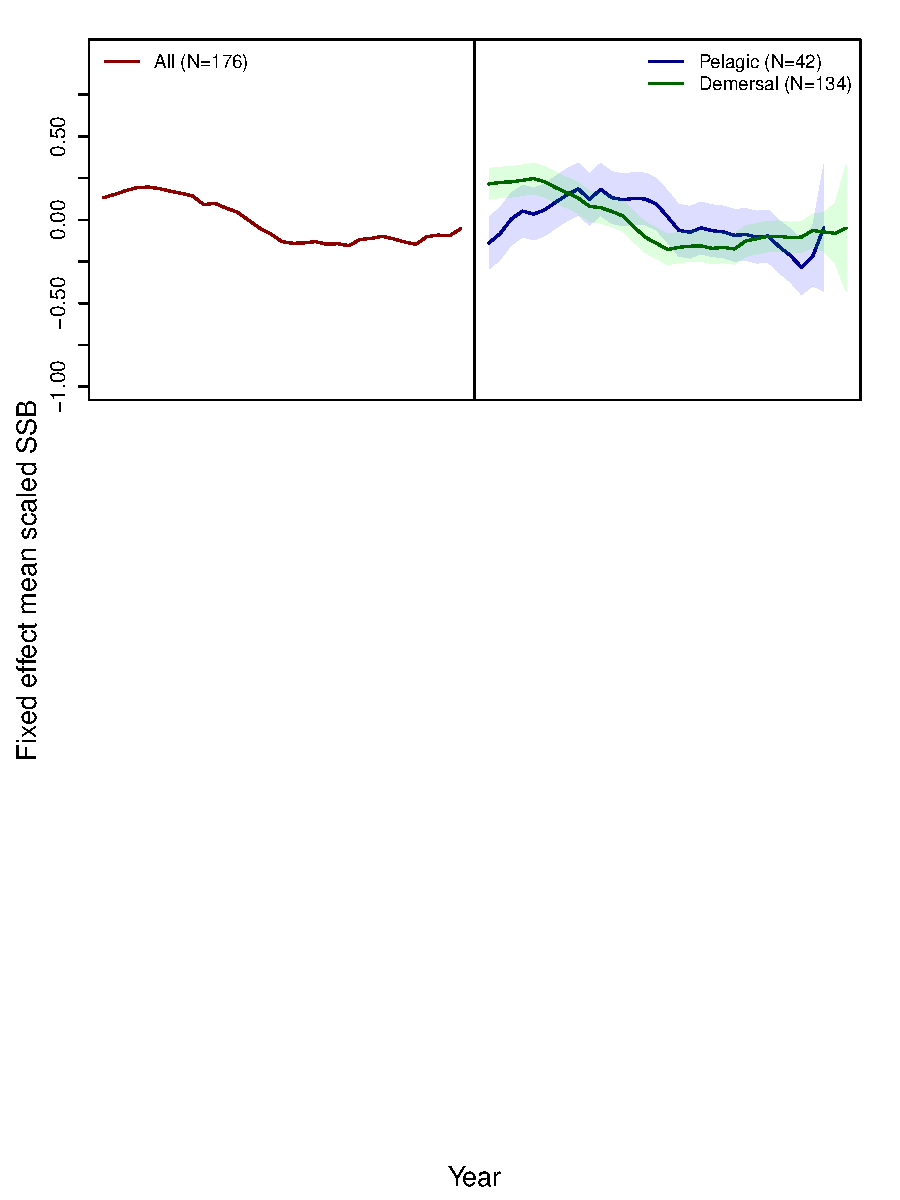
\includegraphics[height=15cm]{/home/srdbadmin/SQLpg/srdb/trunk/projects/baumhutchings/R/Fig2_mixed_effects_alternative.pdf}
\end{center}
\caption{}
\end{figure}\label{fig2}



\end{document}
